\chapter{Industry Experience}
\label{chap:industryExperience}

\section{Introduction}
\label{sec:industryExperience-Introduction}

Business process mining, or process mining for short, aims at the automatic construction of models explaining the behavior observed in the event log \cite{maita2015process}. For example, based on some event log, one can construct a process model expressed in terms of a Petri net.

Over the last couple of years many tools and techniques for process mining have been developed\cite{rozinat2006decision}. Although process mining is very promising, most of the techniques make assumptions which do not hold in practical situations. For example, some techniques assume that there is no noise and have difficulties dealing with exceptions. Other approaches are limited to processes having a particular structure. Therefore, it is important to confront existing tools and techniques with event logs taken from real-life applications.

In this chapter, the business discovery has been experienced using different existing process mining tools(ProM6, Apromore).

\section{Diagnose Problems}

In this chapter, we are going to investigate the problem \#2, as shown in Figure ~\ref{figure:soAndfieldservice}.

This has been used as basis for creating a bpmn diagram capturing the desired process after discussions with members of Highlander.

The resulting process can be seen on \highlight{<link for transaction.bpmn image on google drive>}.

\todo[author=CdS,inline]{Double check names of tasks in the transaction.bpmn file. Make sure each task has number and verb (name of the task must be clear). Generate figure and save in google drive}

\section{Experimental setup}
\label{sec:industryExperience-Methodology}
For this study, we analyzed the data collected from  \textbf{companyA}. 
The original data contains the information about the different roles and employee's name with corresponding time frame. Before introducing the  standard event log (cas ID, activity and time stamp), the NetSuite data will explains


\subsection{NetSuite Events Log Data}
List\ref{lst:sqlNetSuiteAll} shows the SQL extracting all the columns from Transaction table, which includes from sales order to work order, from opportunity to payments and from Bills to return authorisation. The SQL ran for understanding the design of database in NetSuite.

\begin{lstlisting}[language=SQL, caption={comprehensive data SQL}, label={lst:sqlNetSuiteAll} ]
SELECT *
FROM "Transaction"
WHERE RowNum <= 10
\end{lstlisting}

However,  the results of list\ref{lst:sqlNetSuiteAll} contains 453 columns as a CSV file , which is saved in a google doc\footnote{
\url{https://docs.google.com/spreadsheets/d/1Uo6t0si8r36s8oHdHOK50PJxLDHW4PWuQDcRe8V_mN0/edit?usp=sharing}}.
For  easier understanding and explanation, the original data from NetSuite will be cleaned and ignore the unnecessary columns. 

Fig~\ref{figure:saveSearch} shows the "save search" for extracting data from NetSuite, which is equivalent to List~\ref{lst:sqlNetSuite}.  So each Transaction recorded are coded in XLSX format. We collected the instances those are related to all transaction details along with one year time duration. 


\begin{figure}[!htb]
    \centering 
    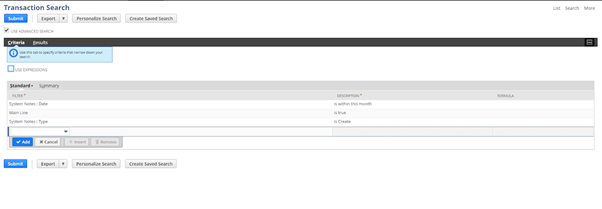
\includegraphics[scale=0.7]{resource/data.png}
    \caption{extracting data interface}
    \label{figure:saveSearch}
\end{figure}



\begin{lstlisting}[language=SQL, caption={equal to SQL}, label={lst:sqlNetSuite} ]
SELECT "Order Type", "Date","Period","Type","Document Number",
    "Name", "System Notes: Set by", "Created From", 
    "Applied to Transaction","Applying Transaction", 
    "System Notes: Role","System Notes: Set by"  
FROM "transaction"
WHERE "SYSTEM NOTE:DATE" 
    WITHIN "01.01.2021" AND 
           "09.02.2022" AND 
    "SYSTEM NOTES: TYPE" == "CREATE"
\end{lstlisting}

In table~\ref{table:dataformat} shows the data in CSV format. 
There are 10000 process instances in the dataset where it shows only the trace 5. There are many activities in trace 5 i.e., Document ID and Period and Created from, timestamp . The trace 1 contains many sequences of activities. Likewise there are 10000 process instances are populated using the transaction activities.

\begin{table}[htb]
\scriptsize %changing the font size
\begin{tabularx}{\textwidth}{|X|X|X|X|X|X|X|X|X|}
\hline
Internal ID & Date & Type & Document Number & Created From & Applied to Transaction & Applying Transaction & Role & Set by\\
\hline
1822448 & 01.02.2021 8:20 AM & Item Receipt & 37308 & Purchase Order \#54527 &  &   & I.T.T. Stock Room & Employee \#1\\
\hline
1822449 & 01.02.2021 8:21 AM & Item Fulfillment & 52882 & Sales Order \#60219 & Sales Order \#60219  &   & I.T.T. Stock Room & Employee \#1\\
\hline
1822454 & 31.01.2021 5:14 PM & Journal & 4672 &	Invoice \#64932 &	Invoice \#64932 &	& Highlander Accountant &	Employee \#2 \\
\hline
\end{tabularx}
\caption{Data Format From NetSuite}
\label{table:dataformat}
\end{table}


Even log contains columns in table~\ref{table:dataformat} from left to right:
\begin{enumerate}
    \item \textbf{Internal ID}: This is the unique ID for each activity from NetSuite database ID.
    \item \textbf{Date}: It is timestamp for activity
    \item \textbf{Type}: The columns show different type of tasks. Those are the tasks that compose the business process.
    \item \textbf{Document Number}: The unique task ID for the particular process instance.
    \item \textbf{Created From}: The columns shows that the task that happened before the current task.
    \item \textbf{Applied to Transaction} (Applying Transaction): The next associated activity.
    \item \textbf{Role}: The role created or triggered the activity.
    \item \textbf{Set by}: The specific employee that performed the activity. The username of that particular user in the system.
\end{enumerate}

% \todo[inline]{Explain all the possible ``types'' (tasks in the NetSuite system) in the text and not in the table. Use the table with only 2 columns.}


\begin{table}[htb]
\footnotesize	 %changing the font size
\begin{tabularx}{\textwidth}{X|X|X}
\hline
\textbf{Terms in Data} & \textbf{Terms in Problem section} & \textbf{Terms in transaction.bpmn} \\
\hline
Column1 & column 2 & column 3 \\
\hline 
 & &  \\
\hline
Bill &  & \\
\hline
Bill Credit  & &  \\
\hline
Bill Payment &  & \\
\hline
Cash Sale  &  & \\
\hline
Cheque  &  & \\
\hline
Estimate  &  & \\
\hline
Invoice  & 10. invoice (task "10). &  \\
\hline
item Fulfillment  & 5. receive the item(task "5) & Item fulfillment \\
\hline
item Receipt  &  & \\
\hline
Journal  &  \\
\hline
Opportunity  &  \\
\hline
Payment  &  \\
\hline
Purchase Order  & 3. raise purchase order(task "4)  \\
\hline
Sales Order  & 1. raise a sales order (task "1)  \\
\hline
Transfer  &  \\
\hline
Return Authorisation  &  \\
\hline
Field Service  & 4. raise field service (task "4)  \\
\hline
\end{tabularx}
\caption{Explanation of all available types in the NetSuite data. A type corresponds to a task in the business process.}
\label{table:terminologyData}
\end{table}
\todo{match the from figure 4.2 terms in the table 4.2} 

To avoid confusion came from using different type names, the term will be used to describe the comprehensive list combining with the "problem" section~\pageref{figure:soAndfieldservice} used terms. The analysis of terminology collected from NetSuite databases and "problem" section~\pageref{figure:soAndfieldservice}, summarized in Table~\ref{table:terminologyData}

In Table~\ref{table:terminologyData} shows the comparison with problems \#2, a number of transaction terms is not matched with problems \#2. However, the main reason has been believe that problem \#2 are simplify the business process for focusing on the process problems rather than the whole process.For explanations,  \href{https://docs.oracle.com/en/cloud/saas/netsuite/ns-online-help/section_4483109897.html}{Oracle} provides the list of transaction type and \href{https://docs.oracle.com/en/cloud/saas/netsuite/ns-online-help/chapter_3794468027.html}{glossary}.



\subsection{Data Preprocessing}
Data preprocessing is the efficient process to discover suitable attributes from the event log. Collection of sequence process in the event are extracted from the source list of activities and mentioned the related events and attributes of log. We have to concentrate important processes to maintain the efficiency in the source data set, i.e.
\begin{enumerate}
    \item Noise
    \item Incompleteness
\end{enumerate}

Noise: The incorrect event logs are removed from the dataset.
While extracting information from event log the various
sources can interleaf the information. The algorithm will
mislead the accuracy of the result. So the non-behavioral
information must be distinguished from the other data set and
retrieve the proper information.
Incompleteness: The unwanted and NAN attributes are produce noise in
the data process and mislead the control flow of the process
mining


In table~\ref{table:datapreprocessed-case1}, we present the result after our data pre-processing.
For example, we are now able to identify the specific case ID (or process instance ID) of the trace log.
In this table we show the trace for case ID 1.

\begin{table}[htb]
\scriptsize %changing the font size
\begin{tabularx}{\textwidth}{|X|X|X|X|X|X|X|X|X|X|}
\hline
Case ID &Internal ID & Date & Type & Document Number & Created From & Applied to Transaction & Applying Transaction & Role & Set by\\
\hline
1 &1825271 & 03.02.2021 1:18 PM & Opportunity & 6423 &   &  &   & I.T.T. Stock Room & Employee \#1\\
\hline
1 &1825240 & 03.02.2021 11:14 AM & Estimate & 70266 & Opportunity \# 6423 & Sales Order \#60637  &   & I.T.T. Stock Room & Employee \#1\\
\hline
1 & 1834387 & 12.02.2021 4:36 PM & Sales Order & 60637 &	Estimate \#6423 &	Purchase Order \#64932 &	& Highlander Accountant &	Employee \#2 \\
\hline
1&1835568 & 12.02.2021 5:08 PM & Purchase Order & 54972 &	Sales Order \#60637
 &	 &	& Highlander Accountant &	Employee \#2 \\
\hline
1&1844081 & 23.02.2021 4:14 PM & Item Fulfillment & 53500 &	Sales Order \#60637
 &	 &	& Highlander Accountant &	Employee \#2 \\
\hline
1&1844080 & 12.02.2021 4:36 PM & Item Receipt & 37912 &	Purchase Order \#54972 &	 &	& Highlander Accountant &	Employee \#2 \\
\hline
1&1844335 & 23.02.2021 9:00 PM & Invoice & 65554 &	Sales Order \#60637
 &	 &	& Highlander Accountant &	Employee \#2 \\
\hline
1&1920910 & 05.05.2021 11:56 AM & Payment & 33907 &	Invoice \#65554
 &	 &	& Highlander Accountant &	Employee \#2 \\
\hline
1&1844326 & 23.02.2021 5:16 PM & Bill & 65554 &	Purchase Order \#54972
 &	 &	& Highlander Accountant &	Employee \#2 \\
\hline
\end{tabularx}
\caption{Pre-processed log data including identification of case id}
\label{table:datapreprocessed-case1}
\end{table}


\begin{table}[htb]
\scriptsize %changing the font size
\begin{tabularx}{\textwidth}{|X|X|X|X|X|X|X|X|X|X|}
\hline
2&1845836 & 24.02.2021 10:26 PM & Estimate & 70949 &	
 &	 &	& I.T. T. Sales Support &	Employee \#3 \\
\hline
2&1848821 & 25.02.2021 9:05 AM & Sales Order  & 61240 &	Estimate \#70949
 &	 &	& I.T. T. Sales Support &	Employee \#2 \\
\hline
2&1855308 & 25.02.2021 9:05 AM & Purchase Order  & 55304 &	Sales Order \#61240
 &	 &	& I.T. T. Sales Support &	Employee \#2 \\
\hline
2&1851320 & 26.02.2021 2:22 PM & Item Fulfillment  & 53616 &	Sales Order \#61240
 &	 &	& Highlander Sales Support Manager &	Employee \#3 \\
\hline
2&1873135 & 19.03.2021 3:02 PM & Invoice  & 66619 &	Sales Order \#61240
 &	 &	& Administrator &	Employee \#4 \\
\hline
2&1851320 & 05.05.2021 9:03 AM & Payment  & 33898 &	Sales Order \#61240
 &	 &	& Highlander Accountant
 &	Employee \#4 \\
\hline
\end{tabularx}
\caption{Raw Data Examples}
\label{table:datapreprocessed-case2}
\end{table}


In our dataset, we have identified 10000 process instances and have taken as the event log. Those one thousand transactions are directed to different events and 12000 events are traced in event history over there. 

The activities are segregated into 20 event classes. 
The mean values of these events are calculated based on cases. Fig~\ref{figure:promXESEvent} shows the number of cases, events and mean value of the given dataset. In 10000 process instances the minimum and maximum values are traces in the Fig~\ref{figure:promXESEvent}. The total traces and by event trace are also mentioned in the diagram. This is the event log visualizer in the process mining. This visualizer helps to see the summary of the activity trace in the process. Log visualizer traces the event which is occurring starting and ending of the process. As well the activity sequence in each trace also identified in this


\begin{figure}[!htb]
    \centering 
    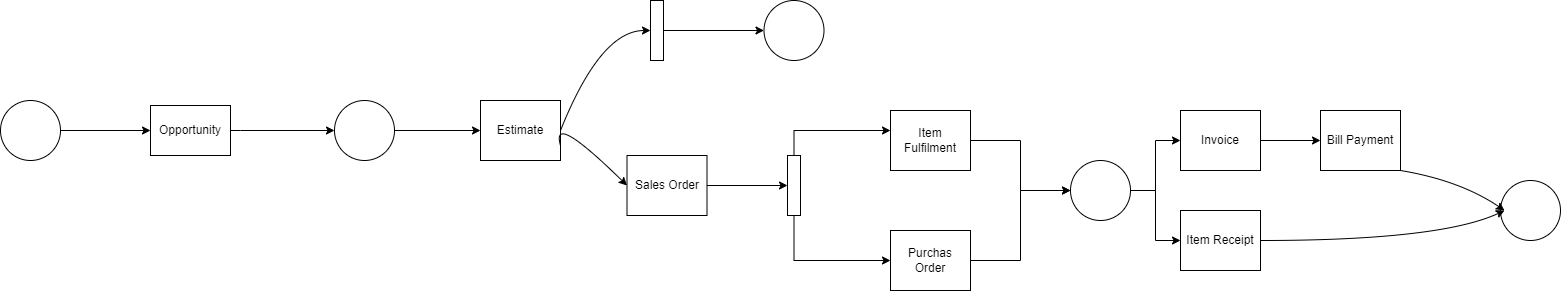
\includegraphics[scale=0.3]{resource/XESeventLog1.png}
    \caption{ProM lite 1.3 XES Event Log Problems}
    \label{figure:promXESEvent}
\end{figure}
\comment[id=CdS]{What is this figure?}


\section{Mining with ProM tool}

This section describes our experiments using the ProM tool.

The information is collected and stored in database, it is important to convert the data into XSLX format. 
ProM will accept the CSV file, so the dataset of other format need to be changed to CSV file format using Python\ref{pythonCode}. 
The CSV extension file is an input to the ProM that has to be imported using the import option. 
The required attributes are selected for process mining like activities and time of the activities. We can filter the attributes which are used particularly in the process.


\subsection{Experiment \#1}

\todo[inline]{Text to describe the experiment using a single case (case ID 1).}

\todo[inline]{Show a table with the preprocessed data for case ID 1}

\todo[inline]{Show a bpmn with the expected result created manually by yourself (considering only case id 1) without looking at ProM tool}

\todo[inline]{Show the result from ProM tool}

\todo[inline]{Text comparing the expected result and obtained result.}

\subsection{Experiment \#2}

\todo[inline]{Text to describe the experiment using two cases (case ID 1 and 2).}

\todo[inline]{Show a table with the preprocessed data for case ID 2. Mention that case ID 1 has been presented in the previous section.}

\todo[inline]{Show a bpmn with the expected result created manually by yourself (considering both case id 1 and 2) without looking at ProM tool}

\todo[inline]{Show the result from ProM tool}

\todo[inline]{Text comparing the expected result and obtained result.}

\subsection{Experiment \#3}

\todo[inline]{Text to describe the experiment using two cases (case ID 1 and 2 and 3).}

\todo[inline]{Show a table with the preprocessed data for case ID 3. Mention that case ID 1 and 2 have been presented in the previous sections.}

\todo[inline]{Show a bpmn with the expected result created manually by yourself (considering both case id 1 and 2 and 3) without looking at ProM tool}

\todo[inline]{Show the result from ProM tool}

\todo[inline]{Text comparing the expected result and obtained result.}

\subsection{Experiment \#4}

\todo[inline]{Text to describe the experiment using ten cases.}

\todo[inline]{preprocessed data for the 10 cases can be saved in a gsheet. Include the link to the gsheet here.}

\todo[inline]{Show a bpmn with the expected result created manually by yourself (considering the 10 cases) without looking at ProM tool}

\todo[inline]{Show the result from ProM tool}

\todo[inline]{Text comparing the expected result and obtained result.}

\subsection{Experiment \#5}

\todo[inline]{Text to describe the experiment using all cases from the dataset.}

\todo[inline]{Text describing the dataset. how many events. how many cases are contained after preprocessing. how many transactions.}


\todo[inline]{Show the result from ProM tool}

\todo[inline]{Text reflecting on the experiment.}

\subsection{Preliminary Conclusions}

\todo[inline]{A text with your conclusions after running the five experiments.}


\section{Lost material}

\comment[id=CdS]{These are material that I don't know what it means.}

\subsection{Event Log Traces}


\begin{figure}[!htb]
        \centering 
    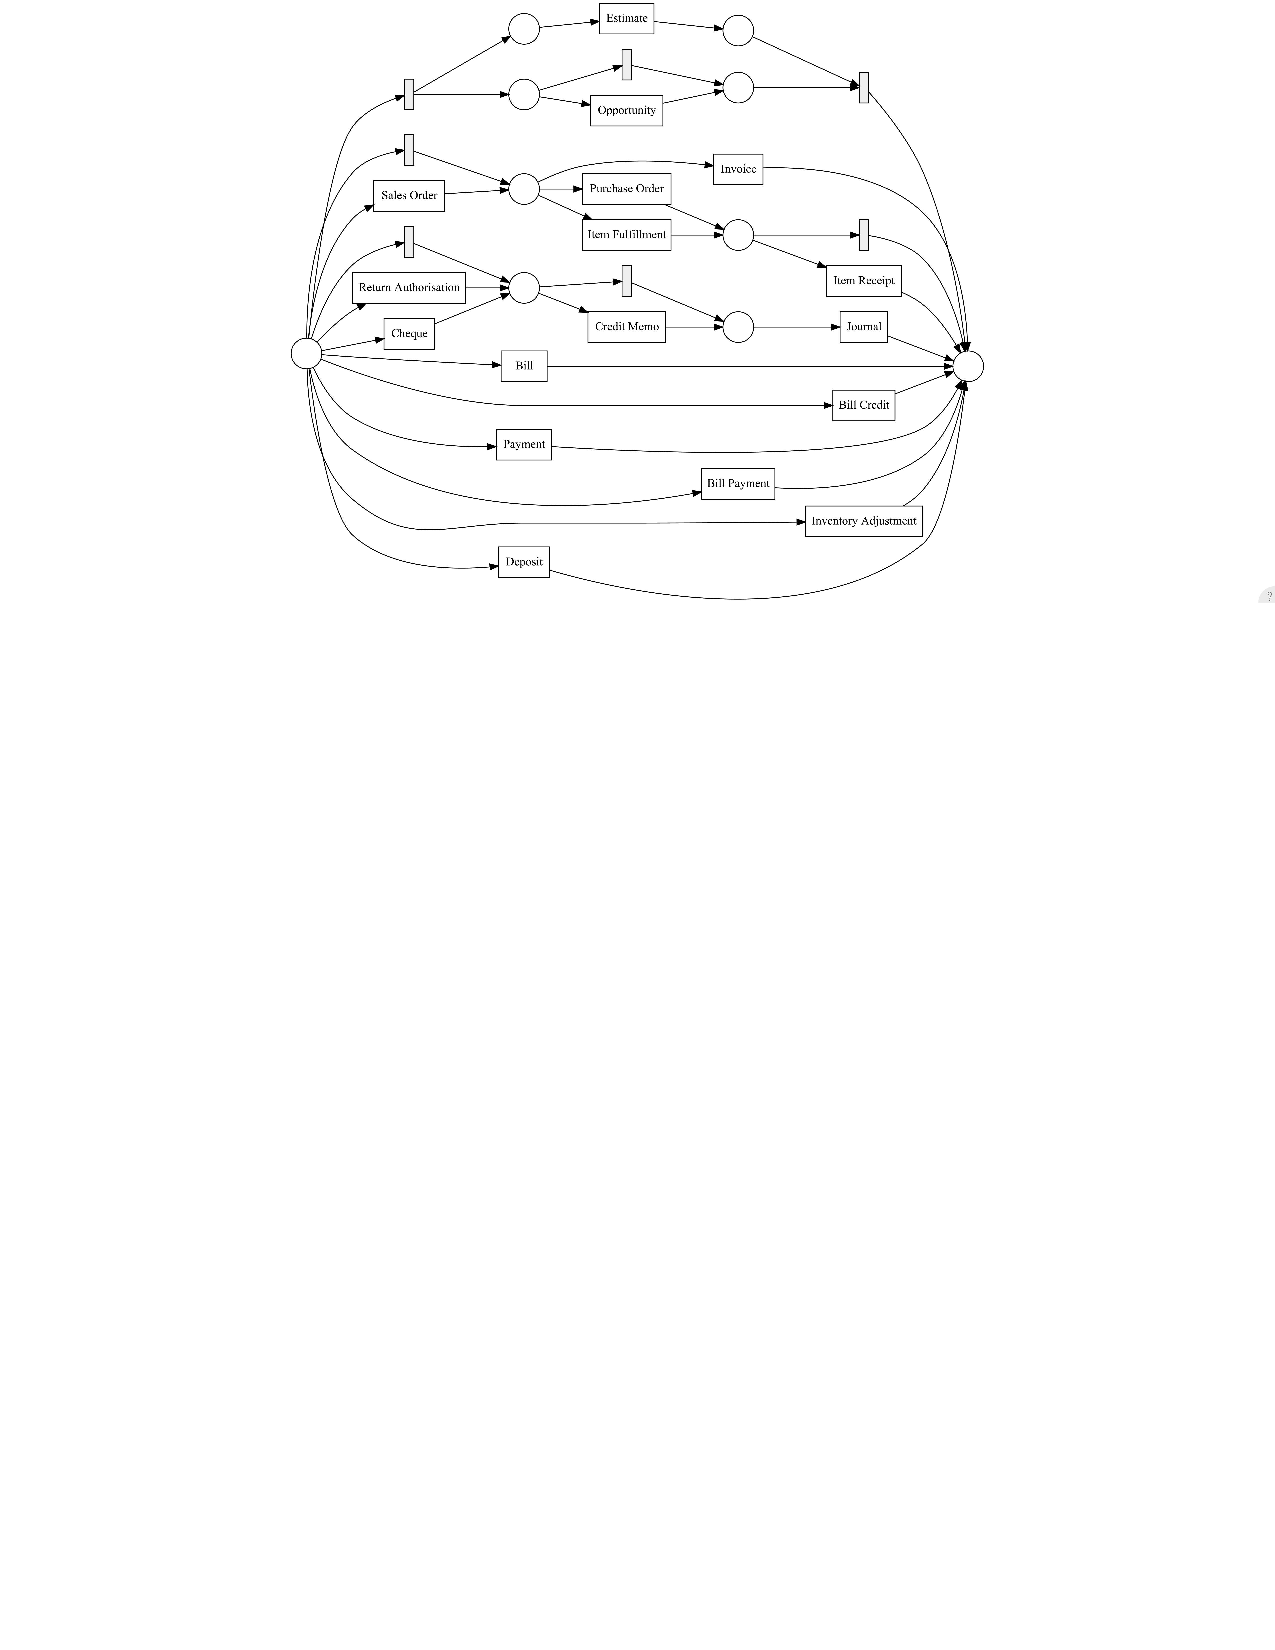
\includegraphics[width =\textwidth, trim =1cm 17cm 0cm 0cm, clip]{resource/problem2.pdf}
    \caption{ProM lite 1.3 Inductive visual Miner}
    \label{figure:eventLogTraces2}

\end{figure}




\subsection{Miner Algorithm}
\todo move to background chapter

\paragraph{Alpha miner}

The alpha-algorithm analyzes the event log to design graphs called patterns. The event log contains the concurrent activities in particular process that means the sequence of activities. The design follows the order of relation in between the activities. Finally alpha algorithm produces the petri net design as result. Our experiment, if activity d is followed by e but vice versa is not possible, then the algorithm confirms dependency relation between d and e. To reflect this dependency, the corresponding Petri net should have a place connecting d to e. We use ordering in between the relations to design the pattern in the event log.

Whenever the complex and frequent activity paths, produces spaghetti[27], that shows the complex structure. The graph determines the activity process flow of patients from start to end. The patient’s details are maintained in admin and the treatment activity and time stamp are mentioned in the process. There are many parallel processes going on and all are noted with time stamp. In alpha algorithm, the entire process will be shown as a graph[28]. Hence, this method which is used for real time applications, such as healthcare process are very helpful to the doctors, hospitals and patients for quick treatment with respect to processing time, waiting time, etc.

\paragraph{The Heuristics miner}
\paragraph{Inductive miner}
\paragraph{Fuzzy miner}






\section{Process mining tools}
\subsection{ProM}
ProM is an extensible framework that supports a wide variety of process mining techniques in the form of plugins. 
It is platform independent as it is implemented in Java, and can be downloaded free of charge. It provides different import data formats, like XES, XML, JSON.
\subsection{Apromore}
Apromore is an open-source process model repository. Its source code is available under the GNU Lesser General Public License.Apromore’s basic features include model import and export, version control and modeling support for a variety of languages, e.g., BPMN,
eEPC, YAWL, and Petri nets. It also supports CSV import. However, they required a format for CSV files 

\section{Source Code}

\todo appendix

\lstinputlisting[language=Python,label={pythonCode},caption=Clean Data Source Code]{resource/Code/cleanData.py}